\PassOptionsToPackage{table}{xcolor}
\documentclass[letterpaper,openany]{book}
\usepackage{enumitem}
\usepackage[en-US,showzone]{datetime2}
\usepackage{fvextra}
\usepackage{float}
\usepackage{graphicx}
\usepackage{hyperref}
\usepackage{listings}
\usepackage{makecell}
\usepackage{multirow}
\usepackage{setspace}
\usepackage{tabularx}
\usepackage{titlesec}
\usepackage{titletoc}
\usepackage{tikz}
\usetikzlibrary{calc,positioning,shapes,decorations.pathreplacing}
\usepackage[T1]{fontenc}
\usepackage[table]{xcolor}
\usepackage[scaled]{beramono}

% \renewcommand{\ttdefault}{beramono}

\renewcommand{\familydefault}{\sfdefault}

\titleformat{\chapter}[display]
            {\normalfont\huge\bfseries}
            {\chaptertitlename~\thechapter}{20pt}{\Huge}

\titlespacing*{\section}{0pt}{1ex}{.1ex}
\titlespacing*{\chapter}{0pt}{1ex}{.1ex}
\titlespacing*{\subsection}{0pt}{1ex}{1ex}
\titlespacing*{\subsubsection}{0pt}{1ex}{1ex}

\titlecontents{chapter}   % Affects chapters
[0em]                    % Left indentation
{}                       % Space before entry
{\bfseries\contentslabel{2.3em}}  % Font for numbered chapters
{}                       % Font for unnumbered chapters
{\titlerule*[1pc]{.}\contentspage}    % Dot leaders
{}          % Page number
\titlecontents{section}   % Affects sections
[1em]                    % Left indentation
{}                       % Space before entry
{\bfseries\contentslabel{2.3em}}  % Font for numbered sections
{}                       % Font for unnumbered sections
{\titlerule*[1pc]{.}\contentspage}    % Dot leaders
{}          % Page number
\titlecontents{subsection}   % Affects subsections
[2.5em]                    % Left indentation
{}                       % Space before entry
{\contentslabel{3.3em}}         % Font for numbered subsections
{}                       % Font for unnumbered subsections
{\titlerule*[1pc]{.}\contentspage}    % Dot leaders
{}          % Page number
\titlecontents{subsubsection}   % Affects subsubsections
[1em]                    % Left indentation
{}                       % Space before entry
{\bfseries}              % Font for numbered subsubsections
{}                       % Font for unnumbered subsubsections
{\titlerule*[1pc]{.}\contentspage}    % Dot leaders
{}          

\textwidth=6.5in
\textheight=9.0in
\oddsidemargin=-0.25in
\evensidemargin=-0.25in
\topmargin=-0.25in
\parskip=1em
\parindent=0in
\itemsep=.1ex

% the styles for short and long nodes
\tikzset{
short/.style={draw,text height=3pt,text depth=20pt,
  text width=7pt,align=center,fill=blue!10},
long/.style={short,fill=green!10,text width=(\textwidth-64pt)/3},
dotdot/.style={fill=white,minimum width=(\textwidth-96pt)/3},
eightByteEmpty/.style={draw,fill=blue!10,text depth=20pt,text width=96pt,align=center},
fourByteEmpty/.style={draw,fill=blue!10,minimum height=20pt,text depth=10pt,text width=48pt,align=center,text centered}}

\makeatletter
    \let\pgf@decorate@@brace@brace@code@old\pgf@decorate@@brace@brace@code
    \def\pgf@decorate@@brace@brace@code{
        \ifdim\pgfdecoratedremainingdistance<4\pgfdecorationsegmentamplitude
            \pgftransformxscale{\pgfdecoratedremainingdistance/4\pgfdecorationsegmentamplitude}
            \pgfdecoratedremainingdistance=4\pgfdecorationsegmentamplitude
        \fi
        \pgf@decorate@@brace@brace@code@old
    }
    \makeatother

% Using Courier font
% \renewcommand{\ttdefault}{pcr}

\definecolor{dwmOrange}{RGB}{255,127,42}
\definecolor{codegray}{rgb}{0.7,0.7,0.7}
\definecolor{codeblue}{rgb}{0.2,0.2,1.0}
\definecolor{darkblue}{rgb}{0.0,0.0,0.7}
\definecolor{green1}{RGB}{0,160,0}
\definecolor{red1}{RGB}{160,0,0}
\definecolor{numberbg}{rgb}{0.9,0.9,0.2}
\definecolor{numbercolor}{rgb}{0.2,0.2,1.0}
\colorlet{mynumberbg}{numberbg!20}
\colorlet{mynumbercolor}{numbercolor!40}

\lstdefinestyle{mystyle}%
{basicstyle=\ttfamily,
 keywordstyle=\ttfamily\color{black},
 identifierstyle=\ttfamily\color{black},
 morekeywords={std::string, cout, cin, vector, map, assert},
 keepspaces=true,
 showspaces=false,                
 showstringspaces=false,
% numberstyle=\sffamily\small\color{codegray},
 numbers=left,                    
 numbersep=1em,
 frame=l,
 framesep=2em,
 framexleftmargin=.8em,
 fillcolor=\color{mynumberbg},
 rulecolor=\color{mynumberbg},
 numberstyle=\sffamily\small\color{mynumbercolor}
}

\lstset{language=C++,
  style=mystyle
}

\newcommand{\conceptfuncsig}[1]{{\color{darkblue}\bfseries\ttfamily #1}}
\newcommand{\conceptfsigpar}[1]{\vspace{.5ex}\begin{itemize}[noitemsep,nolistsep]\item[]\conceptfuncsig{#1}\end{itemize}}

\DefineVerbatimEnvironment{fnverb}{Verbatim}{
  fontfamily=\ttdefault,
  fontshape=\updefault,
  fontseries=bx,
  breaklines,
  breakanywhere,
  breaksymbolleft=,
  breakindent=0pt
}

\hypersetup{
    colorlinks=true,
    linkcolor=blue,
    filecolor=magenta,    
    urlcolor=cyan,
    pdftitle={libDwm I/O},
    pdfpagemode=FullScreen,
}

\begin{document}
\begin{titlepage}
  \begin{center}

    \tikzstyle{mybox} = [draw=white, fill=white!100, thick,
      rectangle, rounded corners, inner sep=10pt, inner ysep=20pt, text=black]
    \begin{tikzpicture}
      \node [mybox] (box){
        \begin{minipage}{0.9\textwidth}
          \begin{Huge}
            \begin{center}
              \resizebox{0.5\linewidth}{!}{libDwm I/O}
            \end{center}
          \end{Huge}
        \end{minipage}
      };
    \end{tikzpicture}

    \resizebox{0.3\linewidth}{!}{Manual}
    
    \vfill

    \color{black}
    \begin{Large}
    Version 1.0.0
    \end{Large}
    
    \color{dwmOrange}
    \rule{\linewidth}{.5mm}
    \color{black}
    
    \tikzstyle{mybox} = [draw=white, fill=white!100, thick,
      rectangle, rounded corners, inner sep=10pt, inner ysep=5pt, text=black]
    \begin{tikzpicture}
      \node [mybox] (box){
        \begin{minipage}{0.9\textwidth}
            \begin{center}
            Copyright \copyright\ 2025 Daniel W. McRobb\linebreak
            Last Revision: \DTMnow
            \end{center}
        \end{minipage}
      };
    \end{tikzpicture}
    
  \end{center}

\end{titlepage}

%% \begin{spacing}{0.0}
\begingroup
\renewcommand{\baselinestretch}{1.0}
\tableofcontents
\endgroup
%% \end{spacing}

\chapter{Introduction}

\section{Motivation}
\begin{description}
\item[Efficiency]  I did not want conversions between textual and native
  representations for arithmetic types.  For example, if I need to stream
  an unsigned 32-bit integer of value 0xFFFFFFFF, I should only need to
  transfer 4 bytes, not 10 or more.
\item[Portability]  Since network transport was a primary goal, I was
  motivated to provide schemes that work across fairly common hardware
  platforms and UNIX operating systems.
\item[Flexibility]  I/O facilities should be flexible enough to accomodate
  instances of common class templates from the standard library, particularly
  containers like \texttt{vector}, \texttt{map}, et. al.  They should
  also be flexible enough to accomodate user-defined types without a
  tremendous amount of work.
\end{description}

\section{History}
libDwm was started around 1998.  Needless to say, C++ was a very
different language in 1998 versus 2025.  And the standard library has
grown tremendously since 1998.

The I/O facilities in libDwm started appearing in the early 2000's
(around the time we got C++03).  Since that time, it has evolved a bit
with each new version of the C++ standard, and is about to see a sea
change with C++26 reflection (P2996 and P3394 in particular).

\section{Primary I/O classes}

\section{Directly supported types}

\section{Supported \texttt{std} class templates}

\section{Concepts}

\chapter{Design}

\section{A primary I/O class for each source/sink type}
The library divides I/O functionality into a primary I/O class
for a given type of source and sink.  For example,
\hyperref[section:DwmStreamIOClass]{\texttt{Dwm::StreamIO}} provides
functions for \texttt{std::istream} sources and \texttt{std::ostream}
sinks.  Table~\ref{table:PrimaryClassSourceSinkType} lists the primary
I/O classes and their associated source and sink type.

\begin{table}[H]
\begin{tabular}{llll}
  \textbf{Primary I/O class} & \textbf{Source type} & \textbf{Sink type} & \textbf{Description} \\ \hline
  \hyperref[section:DwmStreamIOClass]{\texttt{Dwm::StreamIO}} & \texttt{std::istream \&} & \texttt{std::ostream \&} & references to C++ iostreams \\
  \hyperref[section:DwmFileIOClass]{\texttt{Dwm::FileIO}} & \texttt{FILE *} & \texttt{FILE *} & \texttt{FILE} created with \texttt{fopen()} and friends \\
  \hyperref[section:DwmDescriptorIOClass]{\texttt{Dwm::DescriptorIO}} & \texttt{int} & \texttt{int} & UNIX descriptors \\
  \hyperref[section:DwmBZ2IOClass]{\texttt{Dwm::BZ2IO}} & \texttt{BZFILE *} & \texttt{BZFILE *} & \texttt{BZFILE} created with \texttt{BZ2\_bzopen()}\\
  \hyperref[section:DwmGZIOClass]{\texttt{Dwm::GZIO}} & \texttt{gzFile} & \texttt{gzFile} & \texttt{gzFile} created with \texttt{gzopen()} \\
\end{tabular}
\caption{Primary I/O class source and sink types}
\label{table:PrimaryClassSourceSinkType}
\end{table}

Each of the primary I/O classes provides a set of static functions and
function templates to read and write data.

\section{Conceptual interfaces}
Conceptually, the I/O classes provide four primary interfaces to read
and write from/to their associated source/sink type, as depicted in
table~\ref{table:ConceptualInterfaceGeneric}.  There are
single-object interfaces (\texttt{ReadFunc} and \texttt{WriteFunc})
and multi-object variadic interfaces (\texttt{VariadicReadFunc} and
\texttt{VariadicWriteFunc}).  The multi-object variadic interfaces
just call to the single-object interfaces for each object.

\begin{table}[H]
\begin{tabular}{l}
  \textbf{Read/write functions (conceptual)} \\ \hline
  \makecell[l]{\texttt{template <typename T>}\\ \texttt{static \textit{\color{red1}ReadReturnType} \& \color{darkblue}{\textit{ReadFunc}}(\textit{\color{green1}SourceType} {\color{green1}source}, T \& t);}} \\
  \makecell[l]{\texttt{template <typename T>}\\ \texttt{static \textit{\color{red1}WriteReturnType} \textit{\color{darkblue}WriteFunc}(\textit{\color{green1}SinkType} {\color{green1}sink}, const T \& t);}} \\
  \makecell[l]{\texttt{template <typename... Args>}\\ \texttt{static \textit{\color{red1}ReadReturnType} \textit{\color{darkblue}VariadicReadFunc}(\textit{\color{green1}SourceType} {\color{green1}source}, Args \& ...args);}} \\
  \makecell[l]{\texttt{template <typename... Args>}\\ \texttt{static \textit{\color{red1}WriteReturnType} \textit{\color{darkblue}VariadicWriteFunc}(\textit{\color{green1}SinkType} {\color{green1}sink}, const Args \& ...args);}} \\
\end{tabular}
\caption{Conceptual read/write functions in all primary I/O classes}
\label{table:ConceptualInterfaceGeneric}
\end{table}

Table~\ref{table:ConceptualInterfaceMapping} maps the generic conceptual
interface to each of the primary I/O classes.

\begin{table}[H]
\begin{tabular}{l|l|l|l|l|l}
  & \multicolumn{5}{c}{\texttt{Dwm} I/O class} \\
  & \texttt{StreamIO} & \texttt{FileIO} & \texttt{DescriptorIO} & \texttt{BZ2IO} & \texttt{GZIO} \\ \hline
  \texttt{\textit{\color{darkblue}ReadFunc}} & \texttt{\color{darkblue}Read} & \texttt{\color{darkblue}Read} & \texttt{\color{darkblue}Read} & \texttt{\color{darkblue}BZRead} & \texttt{\color{darkblue}Read} \\
  \texttt{\textit{\color{darkblue}VariadicReadFunc}} & \texttt{\color{darkblue}ReadV} & \texttt{\color{darkblue}ReadV} & \texttt{\color{darkblue}ReadV} & \texttt{\color{darkblue}BZReadV} & \texttt{\color{darkblue}ReadV} \\
  \texttt{\textit{\color{red1}ReadReturnType}} & \texttt{\color{red1}std::istream \&} & \texttt{\color{red1}size\_t} & \texttt{\color{red1}ssize\_t} & \texttt{\color{red1}int} & \texttt{\color{red1}int} \\
  \color{green1}\texttt{\textit{SourceType}} & \color{green1}\texttt{std::istream \&} & \color{green1}\texttt{FILE *} & \color{green1}\texttt{int} & \color{green1}\texttt{BZFILE *} & \color{green1}\texttt{gzFile} \\
  \texttt{\textit{\color{darkblue}WriteFunc}} & \texttt{\color{darkblue}Write} & \texttt{\color{darkblue}Write} & \texttt{\color{darkblue}Write} & \texttt{\color{darkblue}BZWrite} & \texttt{\color{darkblue}Write} \\
  \texttt{\textit{\color{darkblue}VariadicWriteFunc}} & \texttt{\color{darkblue}WriteV} & \texttt{\color{darkblue}WriteV} & \texttt{\color{darkblue}WriteV} & \texttt{\color{darkblue}BZWriteV} & \texttt{\color{darkblue}WriteV} \\
  \texttt{\textit{\color{red1}WriteReturnType}} & \texttt{\color{red1}std::ostream \&} & \texttt{\color{red1}size\_t} & \texttt{\color{red1}ssize\_t} & \texttt{\color{red1}int} & \texttt{\color{red1}int} \\
  \texttt{\textit{\color{green1}SinkType}} & \texttt{\color{green1}std::ostream \&} & \texttt{\color{green1}FILE *} & \texttt{\color{green1}int} & \texttt{\color{green1}BZFILE *} & \texttt{\color{green1}gzFile} \\
\end{tabular}
\caption{Conceptual interface mapping to the primary I/O classes}
\label{table:ConceptualInterfaceMapping}
\end{table}

\section{Categories of interface overloads in actual implementation}
There are three categories of overloads in the implementation:
\begin{itemize}[noitemsep,nolistsep]
\item Regular functions for directly supported types
\item Function templates for STL containers and other standard class
  templates
\item Function templates for types that meet the conceptual requirements
  of a given \hyperref[chapter:primaryIOClasses]{primary I/0 class}
\end{itemize}

\subsection{Regular functions for directly supported types}
Reading and writing of directly supported types is done with regular
function overloads.  For example, this function from
\hyperref[section:DwmStreamIOClass]{\texttt{Dwm::StreamIO}}
to write a \texttt{uint32\_t} value:
\begin{verbatim}
  static std::ostream & Write(std::ostream & os, uint32_t value);
\end{verbatim}

\subsection{Function templates for STL containers and other standard class templates}
Overloaded function templates are used to read and write instantiations of
standard class templates, where the parameter types of the standard
class templates are either directly supported types, types that meet
the conceptual requirements of a readable and writable class, or instances
of supported standard templates using any of the aforementioned types in
type parameters.  In other words, supported standard containers of any depth
can be read and written, as long as the leaf types are directly
supported types or types that meet the conceptual requirements of a
readable and writable class for the I/O class of interest.

This is probably best explained via some example readable and writable
types:
\begin{verbatim}
  std::vector<std::string>
  std::map<uint32_t,std::vector<std::string>>
  std::map<uint32_t,std::vector<std::map<uint8_t,std::string>>>
\end{verbatim}

An example of one such function template from
\hyperref[section:DwmStreamIOClass]{\texttt{Dwm::StreamIO}}:

\begin{verbatim}
    template <typename valueT, size_t N>
    static std::istream & Read(std::istream & is, std::array<valueT, N> & a)
\end{verbatim}

\subsection{Function templates for types that meet the conceptual requirements of a given primary I/O class}
Overloaded function templates with concept requirements are used to read
and write types that meet the concept requirements.  The concepts required
for each primary I/O class are listed in
table~\ref{table:PrimaryIOClassConcepts}.

An example of one such function template from
\hyperref[section:DwmStreamIOClass]{\texttt{Dwm::StreamIO}}:

\begin{ttfamily}
  static std::ostream \& Write(std::ostream \& os, const \hyperlink{concept:HasStreamWrite}{HasStreamWrite} auto \& t)
\end{ttfamily}

\begin{table}[H]
\begin{tabular}{lll}
  \textbf{\texttt{Dwm} I/O class} & \textbf{Read concept} & \textbf{Write concept} \\ \hline
  \hyperref[section:DwmStreamIOClass]{\texttt{StreamIO}} & \hyperlink{concept:HasStreamRead}{\texttt{Dwm::HasStreamRead<T>}} & \hyperlink{concept:HasStreamWrite}{\texttt{Dwm::HasStreamWrite<T>}} \\
  \hyperref[section:DwmFileIOClass]{\texttt{FileIO}} & \hyperlink{concept:HasFileRead}{\texttt{Dwm::HasFileRead<T>}} & \hyperlink{concept:HasFileWrite}{\texttt{Dwm::HasFileWrite</t>}} \\
  \hyperref[section:DwmDescriptorIOClass]{\texttt{DescriptorIO}} & \hyperlink{concept:HasDescriptorRead}{\texttt{Dwm::HasDescriptorRead<T>}} & \hyperlink{concept:HasDescriptorWrite}{\texttt{Dwm::HasDescriptorWrite<T>}} \\
  \hyperref[section:DwmBZ2IOClass]{\texttt{BZ2IO}} & \hyperlink{concept:HasBZRead}{\texttt{Dwm::HasBZRead<T>}} & \hyperlink{concept:HasBZWrite}{\texttt{Dwm::HasBZWrite<T>}} \\
  \hyperref[section:DwmGZIOClass]{\texttt{GZIO}} & \hyperlink{concept:DwmHasGZRead}{\texttt{Dwm::HasGZRead<T>}} & \hyperlink{concept:DwmHasGZWrite}{\texttt{Dwm::HasGZWrite<T>}} \\
\end{tabular}
\caption{Primary I/O class concepts for user-defined types}
\label{table:PrimaryIOClassConcepts}
\end{table}

\section{\texttt{Dwm::StreamIO} read/write functions}
\subsection{\texttt{Dwm::StreamIO} conceptual read/write functions}
Table ~\ref{table:StreamIOConceptualReadWriteFuncs} lists the conceptual
read and write member functions in \texttt{Dwm::StreamIO}.
\begin{table}[H]
\begin{tabular}{ll}
  \textbf{Primary I/O class} & \textbf{Read/write functions (conceptual)} \\ \hline
  \multirow{4}{*}{\hyperref[section:DwmStreamIOClass]{\texttt{Dwm::StreamIO}}} & \makecell[l]{\texttt{template <typename T>}\\ \texttt{static std::istream \& Read(std::istream \& is, T \& t);}} \\ \cline{2-2}
  & \makecell[l]{\texttt{template <typename T>}\\ \texttt{static std::ostream \& Write(std::ostream \& os, const T \& t);}} \\ \cline{2-2}
  & \makecell[l]{\texttt{template <typename... Args>}\\ \texttt{static std::istream \& ReadV(std::istream \& is, Args \& ...args);}} \\ \cline{2-2}
  & \makecell[l]{\texttt{template <typename... Args>}\\ \texttt{static std::ostream \& WriteV(std::ostream \& os, const Args \& ...args);}} \\ \hline
\end{tabular}
\caption{Conceptual read and write member functions in \texttt{Dwm::StreamIO}}
\label{table:StreamIOConceptualReadWriteFuncs}
\end{table}

\begin{minipage}{\textwidth}
Conceptually...

\subsubsection{\texttt{template <typename T>}\\ \texttt{static std::istream \& Read(std::istream \& is, T \& t)}}
\begin{itemize}[noitemsep,nolistsep]
\item Reads the contents of \texttt{t} from \texttt{is} and returns
  \texttt{is}.
\end{itemize}

\subsubsection{\texttt{template <typename T>}\\ \texttt{static std::Write(std::ostream \& os, const T \& t)}}
\begin{itemize}[noitemsep,nolistsep]
\item Writes the contents of \texttt{t} to \texttt{os} and returns
  \texttt{os}.
\end{itemize}

\subsubsection{\texttt{template <typename... Args>}\\ \texttt{static std::istream \& ReadV(std::istream \& is, Args \& ...args)}}
\begin{itemize}[noitemsep,nolistsep]
\item Reads the contents of all \texttt{args} (in order) from \texttt{is}
  and returns \texttt{is}.
\end{itemize}

\subsubsection{\texttt{template <typename... Args>}\\ \texttt{static std::ostream \& WriteV(std::ostream \& os, const Args \& ...args)}}
\begin{itemize}[noitemsep,nolistsep]
\item Writes the contents of all \texttt{args} (in order) to \texttt{os}
  and returns \texttt{os}.
\end{itemize}

\end{minipage}

\section{\texttt{Dwm::FileIO} read/write functions}
\subsection{\texttt{Dwm::FileIO} conceptual read/write functions}
\begin{tabular}{ll}
  \textbf{Primary I/O class} & \textbf{Read/write functions (conceptual)} \\ \hline  \multirow{4}{*}{\hyperref[section:DwmFileIOClass]{\texttt{Dwm::FileIO}}} & \makecell[l]{\texttt{template <typename T>}\\ \texttt{static size\_t Read(FILE *f, T \& t);}} \\ \cline{2-2}
  & \makecell[l]{\texttt{template <typename T>}\\ \texttt{static size\_t Write(FILE *f, const T \& t);}} \\ \cline{2-2}
  & \makecell[l]{\texttt{template <typename... Args>}\\ \texttt{static size\_t ReadV(FILE *f, Args \& ...args);}} \\ \cline{2-2}
  & \makecell[l]{\texttt{template <typename... Args>}\\ \texttt{static size\_t WriteV(FILE *f, const Args \& ...args);}} \\ \hline
\end{tabular}

\section{\texttt{Dwm::DescriptorIO} read/write functions}
\subsection{\texttt{Dwm::DescriptorIO} conceptual read/write functions}
\begin{tabular}{ll}
  \textbf{Primary I/O class} & \textbf{Read/write functions (conceptual)} \\ \hline
  \multirow{2}{*}{\hyperref[section:DwmDescriptorIOClass]{\texttt{Dwm::DescriptorIO}}} & \makecell[l]{\texttt{template <typename T>}\\ \texttt{static ssize\_t Read(int fd, T \& t);}} \\ \cline{2-2}
  & \makecell[l]{\texttt{template <typename T>}\\\texttt{static ssize\_t Write(int fd, const T \& t);}} \\ \cline{2-2}
  & \makecell[l]{\texttt{template <typename... Args>}\\ \texttt{static ssize\_t ReadV(int fd, Args \& ...args);}} \\ \cline{2-2}
  & \makecell[l]{\texttt{template <typename... Args>}\\ \texttt{static ssize\_t WriteV(int fd, const Args \& ...args);}} \\ \hline
\end{tabular}

\section{\texttt{Dwm::BZ2IO} read/write functions}
\subsection{\texttt{Dwm::BZ2IO} conceptual read/write functions}
\begin{tabular}{ll}
  \textbf{Primary I/O class} & \textbf{Read/write functions (conceptual)} \\ \hline
  \multirow{2}{*}{\hyperref[section:DwmBZ2IOClass]{\texttt{Dwm::BZ2IO}}} & \makecell[l]{\texttt{template <typename T>}\\ \texttt{static int BZRead(BZFILE *bzf, T \& t);}} \\ \cline{2-2}
  & \makecell[l]{\texttt{template <typename T>}\\ \texttt{static int BZWrite(BZFILE *bzf, const T \& t)}} \\ \cline{2-2}
 & \makecell[l]{\texttt{template <typename... Args>}\\ \texttt{static int BZReadV(BZFILE *bzf, Args \& ...args);}} \\ \cline{2-2}
  & \makecell[l]{\texttt{template <typename T>}\\ \texttt{static int BZWriteV(BZFILE *bzf, const Args \& ...args)}} \\ \hline
\end{tabular}

\section{\texttt{Dwm::GZIO} read/write functions}
\subsection{\texttt{Dwm::GZIO} conceptual read/write functions}
\begin{tabular}{ll}
  \textbf{Primary I/O class} & \textbf{Read/write functions (conceptual)} \\ \hline
  \multirow{2}{*}{\hyperref[section:DwmGZIOClass]{\texttt{Dwm::GZIO}}} & \makecell[l]{\texttt{template <typename T>}\\ \texttt{static int Read(gzFile gzf, T \& t);}} \\ \cline{2-2}
  & \makecell[l]{\texttt{template <typename T>}\\ \texttt{static int Write(gzFile gzf, const T \& t);}} \\ \cline{2-2}
 & \makecell[l]{\texttt{template <typename... Args>}\\ \texttt{static int ReadV(gzFile gzf, Args \& ...args);}} \\ \cline{2-2}
  & \makecell[l]{\texttt{template <typename... Args>}\\ \texttt{static int Write(gzFile gzf, const Args \& ...args);}} \\ \hline
\end{tabular}

\section{Member function overloads}
libDwm uses member function overloading to allow the user to use the
same function names to read or write different types from/to a
source/sink.  This is also critical to supporting instances of class
templates.

\section{Member function templates}
libDwm uses function templates and function template overloads to
provide the same interfaces (the same member function names) to
read or write instances of standard class templates from/to a
source/sink (\texttt{std::vector}, \texttt{std::pair},
\texttt{std::tuple}, \texttt{std::map}, et. al.).

\section{Concepts}
libDwm uses concepts in many places to aid in overload resolution
and to document the requirements of user-defined types.

\section{Support for user-designed types}
\subsection{Before C++26}
In general, code utilized with pre-C++26 compilers and standard libraries
requires a pair of member functions to be added to any user-defined type
for a given source/sink pair.  Much of the time, these functions are
fairly simple to implement, particuarly for C++ iostreams
(\texttt{std::istream} as a source, \texttt{std::ostream} as a sink).
This is especially true for user-defined types that only contain types
already supported by the corresponding primry I/O class (for C++ iostreams,
that would be \texttt{Dwm::StreamIO}).

\subsection{C++26 and beyond}
With C++26 features (particularly P2996 and P3394), it becomes possible
to elegantly handle serialization and deserialization of many user
defined types with no changes to user code.  It also allows annotations
of types and variables that can control the serialization and
deserialization of a user defined type (for example, skipping a data
member of a class during serialization and deserialization).  Work
here has already begun, using a slightly modified fork of the bloomberg
clang implementation.

\chapter{Examples}

\section{Write and read a {\ttfamily string} to/from an {\ttfamily iostream}}
The program below writes a {\ttfamily std::string} to a {\ttfamily
  std::stringstream}, then reads a {\ttfamily std::string} from the
{\ttfamily std::stringstream}.  The program in
listing~\ref{listing:example01} returns {\ttfamily 0} if the
string we read matches the string we wrote.

\begin{minipage}{\textwidth}
\lstinputlisting[language=c++,captionpos=b,caption={Write and read a \texttt{string} to/from an \texttt{iostream}},label={listing:example01}]{examples/Example01_HelloWorldString.cc}
\end{minipage}

\pagebreak
\section{Write and read a {\ttfamily map<string,string>} to/from an {\ttfamily iostream}}
The program in listing~\ref{listing:example02} writes a
{\ttfamily std::map<std::string,std::string>} to a
{\ttfamily std::stringstream}, then reads a
{\ttfamily std::map<std::string,std::string>} from the
{\ttfamily std::stringstream} and returns {\ttfamily 0} if the map
we read matches the map we wrote.  This is an example of our support
for standard containers holding supported types ({\ttfamily std::string}
is an explicitly supported type).

\begin{minipage}{\textwidth}
\lstinputlisting[language=c++,captionpos=b,caption={Write and read a \texttt{map<string,string>} to/from an \texttt{iostream}},label={listing:example02}]{examples/Example02_StringMap.cc}
\end{minipage}

% \pagebreak
% \begin{minipage}{\textwidth}
% \lstinputlisting[language=c++]{examples/Example05_StringMap.cc}
% \end{minipage}

\pagebreak
\section{Turtles all the way down}
The program in listing~\ref{listing:example03} writes a
{\ttfamily std::map<std::string,std::vector<std::string>>}
to a {\ttfamily std::stringstream}, then reads a
{\ttfamily std::map<std::string,std::vector<std::string>>} from the
{\ttfamily std::stringstream} and returns {\ttfamily 0} if the map
we read matches the map we wrote.  This is an example of our support
for standard containers and supported types being ``turtles all the
way down'': our support is recursive to any depth.

\begin{minipage}{\textwidth}
  \lstinputlisting[language=c++,captionpos=b,caption={Write and read a \texttt{map<string,vector<string>>} to/from an \texttt{iostream}},label={listing:example03}]{examples/Example03_MapVectorString.cc}
\end{minipage}

\pagebreak
\section{Integrating a user-defined type}
Listing~\ref{listing:example06_preIO} shows a user defined type
\texttt{MyType} with three simple data members: \texttt{id}, \texttt{name}
and \texttt{category}.

\begin{minipage}{\textwidth}
  \lstinputlisting[language=c++,captionpos=b,caption={\texttt{MyType} without explicit \texttt{Dwm::StreamIO} support},label={listing:example06_preIO}]{examples/Example06_UserDefinedType1_PreIOMyType.hh}
\end{minipage}

\subsection{With C++26 reflection}
With C++26 reflection, all of the
\hyperref[chapter:primaryIOClasses]{primary I/O classes} can read and write
instances of \texttt{MyType} from/to their associated source/sink with no
changes to \texttt{MyType}.  The primary I/O classes will do what one would
expect: read and write each of the members of \texttt{MyType}, in the order
in which they appear in the declaration of \texttt{MyType}.

\subsection{Without C++26 reflection}
Without C++26 reflection, two members need to be added to \texttt{MyType}
for each \hyperref[chapter:primaryIOClasses]{primary I/O class} you wish
to use with \texttt{MyType}.  For example,
listing~\ref{listing:example06_postIO} adds support for \texttt{Dwm::StreamIO}
by adding the \texttt{Read(std::istream \&)} and
\texttt{Write(std::ostream \&) const} member functions for the case where
C++26 reflection is not available (\texttt{DWM\_CAN\_USE\_REFLECTION}
is notdefined).  Note that these member functions are simple in this case
because our member data types are all already supported by
\texttt{Dwm::StreamIO} and hence we can use the \texttt{ReadV()} and
\texttt{WriteV()} members of \texttt{Dwm::StreamIO} to implement these
members.

\begin{minipage}{\textwidth}
  \lstinputlisting[language=c++,captionpos=b,caption={\texttt{MyType} with explicit \texttt{Dwm::StreamIO} support when needed},label={listing:example06_postIO}]{examples/Example06_UserDefinedType1_PostIOMyType.hh}
\end{minipage}

\pagebreak
\subsection{A test program to write and read \texttt{std::vector<MyType>}}
The program in listing~\ref{listing:example06} utilizes a user-defined type
\texttt{MyType} that has explicit
\hyperref[section:DwmStreamIOClass]{\texttt{Dwm::StreamIO}} functionality as
needed.  \texttt{MyType} meets the requirements of the
\hyperlink{concept:HasStreamRead}{\texttt{HasStreamRead<T>}}
and
\hyperlink{concept:HasStreamWrite}{\texttt{HasStreamWrite<T>}}
concepts by providing the \texttt{Read(std::istream \&)} member at lines
10-11 and the \texttt{Write(std::ostream \&) const} member at lines 13-14
when we do not have C++26 reflection.

\begin{minipage}{\textwidth}
  \lstinputlisting[language=c++,captionpos=b,caption={Integrating a user-defined type},label={listing:example06}]{examples/Example06_UserDefinedType1_PostIOMain.cc}
\end{minipage}

The main function creates a vector of \texttt{MyType} named \texttt{myvec1}
on line 23.  It writes \texttt{myvec1} to the \texttt{stringstream} named
\texttt{ss} at line 29.  It then creates a second vector of \texttt{MyType}
named \texttt{myvec2} on line 30 and reads the contents of \texttt{myvec2}
from \texttt{ss} on line 31.  On line 32 it checks if the vector we
read (\texttt{myvec2}) matches the vector we wrote (\texttt{myvec1}).

\pagebreak
\subsection{Skipping data when using C++26 reflection}

\chapter{Primary I/O Classes}

\begin{minipage}{\textwidth}
\section{\ttfamily Dwm::StreamIO}
\begin{tabular}{ll}
  source type: & {\ttfamily std::istream} \\
  sink type: & {\ttfamily std::ostream} \\
\end{tabular}
\vspace{1ex}

Uses the \hyperlink{concept:HasStreamRead}{\ttfamily HasStreamRead} and
\hyperlink{concept:HasStreamWrite}{\ttfamily HasStreamWrite} concepts
to detect the presence of stream I/O support within a user defined type.
In the absence of C++26 reflection, this support requires a user defined
type to contain these two member functions:
\vspace{1ex}

\begin{itemize}[noitemsep,nolistsep]
\item[] \conceptfuncsig{std::istream \& Read(std::istream \& is)}
\item[] \conceptfuncsig{std::ostream \& Write(std::ostream \& os) const}
\end{itemize}
\end{minipage}

\begin{minipage}{\textwidth}
\section{\ttfamily Dwm::FileIO}
\begin{tabular}{ll}
  source type: & {\ttfamily FILE *} \\
  sink type: & {\ttfamily FILE *} \\
\end{tabular}
\vspace{1ex}

Uses the \hyperlink{concept:HasFileRead}{\ttfamily HasFileRead} and
\hyperlink{concept:HasFileWrite}{\ttfamily HasFileWrite} concepts to detect
the presence of C stdio support (reading and writing from/to
{\ttfamily FILE *}) in a user defined type.
\vspace{1ex}

\begin{itemize}[noitemsep,nolistsep]
\item[] \conceptfuncsig{size\_t Read(FILE *f)}
\item[] \conceptfuncsig{size\_t Write(FILE *f) const}
\end{itemize}
\end{minipage}

\begin{minipage}{\textwidth}
\section{\ttfamily Dwm::DescriptorIO}
\begin{tabular}{ll}
  source type: & {\ttfamily int} \\
  sink type: & {\ttfamily int} \\
\end{tabular}
\vspace{1ex}

Uses the \hyperlink{concept:HasDescriptorRead}{\ttfamily HasDescriptorRead}
and \hyperlink{concept:HasDescriptorWrite}{\ttfamily HasDescriptorWrite}
concepts to detect the presence of descriptor I/O support (reading and
writing from/to UNIX file descriptors) inside a user defined type.
\vspace{1ex}

\begin{itemize}[noitemsep,nolistsep]
\item[] \conceptfuncsig{ssize\_t Read(int fd)}
\item[] \conceptfuncsig{ssize\_t Write(int fd) const}
\end{itemize}
\end{minipage}

\begin{minipage}{\textwidth}
\section{\ttfamily Dwm::BZ2IO}
\begin{tabular}{ll}
  source type: & {\ttfamily BZFILE *} \\
  sink type: & {\ttfamily BZFILE *} \\
\end{tabular}
\vspace{1ex}

Uses the \hyperlink{concept:HasBZRead}{\ttfamily HasBZRead}
and \hyperlink{concept:HasBZWrite}{\ttfamily HasBZWrite}
concepts to detect the presence of bzip2 I/O support (reading and
writing from/to {\ttfamily BZFILE *}) inside a user defined type.
\vspace{1ex}

\begin{itemize}[noitemsep,nolistsep]
\item[] \conceptfuncsig{int BZRead(BZFILE *)}
\item[] \conceptfuncsig{int BZWrite(BZFILE *) const}
\end{itemize}
\end{minipage}

\begin{minipage}{\textwidth}
\section{\ttfamily Dwm::GZIO}
{\ttfamily gzFile}
\begin{tabular}{ll}
  source type: & {\ttfamily gzFile} \\
  sink type: & {\ttfamily gzFile} \\
\end{tabular}
\vspace{1ex}

\vspace{1ex}
\begin{itemize}[noitemsep,nolistsep]
\item[] \conceptfuncsig{int Read(gzFile)}
\item[] \conceptfuncsig{int BZWrite(gzFile) const}
\end{itemize}
\end{minipage}

\section{\ttfamily Dwm::ASIO}
Boost asio sockets


\chapter{Directly supported data types}\label{ch:dsdt}
Directly supported data types are those types for which we have static
member functions to read the type from a source and write the type to
a sink.  These types include integral types, floating point types,
enumerated types, {\ttfamily std::string} and
{\ttfamily std::vector<bool>}.

\section{integral types}

The category of types for which {\ttfamily std::is\_integral\_v<T>}
evaluates to {\ttfamily true}.

For multi-byte types in this category, we use an MSB-first representation
on-the-wire.

\section{floating point types}

The category of types for which {\ttfamily std::is\_floating\_point\_v<T>}
evaluates to {\ttfamily true}.

We use XDR for the on-the-wire representation of {\ttfamily float} and
{\ttfamily double}.

\section{enumerated types}

The category of types for which {\ttfamily std::is\_enum\_v<T>} evaluates
to {\ttfamily true}.
        
\section{\ttfamily std::string}

\section{\ttfamily std::vector<bool>}


\chapter{Supported {\ttfamily std} type templates}

\begin{minipage}{\textwidth}
\section{\ttfamily std::array<class T, std::size\_t N>}

We can stream any instances of \texttt{std::array<T,N>} where
\texttt{T} satisfies the read and write concepts of the desired
primary I/O class.
\vspace{1ex}

\begin{tabular}{lll}
  \textbf{primary I/O class} & \textbf{Read concept} & \textbf{Write concept} \\ \hline
  \hyperref[section:DwmStreamIOClass]{\texttt{Dwm::StreamIO}} & \hyperref[concept:DwmIsStreamReadable]{\texttt{Dwm::IsStreamReadable<T>}} & \hyperref[concept:DwmIsStreamWritable]{\texttt{Dwm::IsStreamWritable<T>}} \\
  \hyperref[section:DwmFileIOClass]{\texttt{Dwm::FileIO}} & \hyperref[concept:DwmIsFileReadable]{\texttt{Dwm::IsFileReadable<T>}} & \hyperref[concept:DwmIsFileWritable]{\texttt{Dwm::IsFileWritable<T>}} \\
  \hyperref[section:DwmDescriptorIOClass]{\texttt{Dwm::DescriptorIO}} & \hyperref[concept:DwmIsDescriptorReadable]{\texttt{Dwm::IsDescriptorReadable<T>}} & \hyperref[concept:DwmIsDescriptorWritable]{\texttt{Dwm::IsDescriptorWritable<T>}} \\
  \hyperref[section:DwmBZ2IOClass]{\texttt{Dwm::BZ2IO}} & \hyperref[concept:DwmIsBZ2Readable]{\texttt{Dwm::IsBZ2Readable<T>}} & \hyperref[concept:DwmIsBZ2Writable]{\texttt{Dwm::IsBZ2Writable<T>}} \\
  \hyperref[section:DwmGZIOClass]{\texttt{Dwm::GZIO}} & \hyperref[concept:DwmIsGZReadable]{\texttt{Dwm::IsGZReadable<T>}} & \hyperref[concept:DwmIsGZWritable]{\texttt{Dwm::IsGZWritable<T>}} \\
\end{tabular}
\end{minipage}

\begin{minipage}{\textwidth}
\section{\ttfamily std::atomic<class T>}
We can stream any instances of \texttt{std::atomic<T>} where
\texttt{T} satisfies the read and write concepts of the desired
primary I/O class.  Note this excludes cases where T is a raw
pointer, \texttt{std::shared\_ptr} or \texttt{std::weak\_ptr}.
\vspace{1ex}

\begin{tabular}{lll}
  \textbf{primary I/O class} & \textbf{Read concept} & \textbf{Write concept} \\ \hline
  \hyperref[section:DwmStreamIOClass]{\texttt{Dwm::StreamIO}} & \hyperref[concept:DwmIsStreamReadable]{\texttt{Dwm::IsStreamReadable<T>}} & \hyperref[concept:DwmIsStreamWritable]{\texttt{Dwm::IsStreamWritable<T>}} \\
  \hyperref[section:DwmFileIOClass]{\texttt{Dwm::FileIO}} & \hyperref[concept:DwmIsFileReadable]{\texttt{Dwm::IsFileReadable<T>}} & \hyperref[concept:DwmIsFileWritable]{\texttt{Dwm::IsFileWritable<T>}} \\
  \hyperref[section:DwmDescriptorIOClass]{\texttt{Dwm::DescriptorIO}} & \hyperref[concept:DwmIsDescriptorReadable]{\texttt{Dwm::IsDescriptorReadable<T>}} & \hyperref[concept:DwmIsDescriptorWritable]{\texttt{Dwm::IsDescriptorWritable<T>}} \\
  \hyperref[section:DwmBZ2IOClass]{\texttt{Dwm::BZ2IO}} & \hyperref[concept:DwmIsBZ2Readable]{\texttt{Dwm::IsBZ2Readable<T>}} & \hyperref[concept:DwmIsBZ2Writable]{\texttt{Dwm::IsBZ2Writable<T>}} \\
  \hyperref[section:DwmGZIOClass]{\texttt{Dwm::GZIO}} & \hyperref[concept:DwmIsGZReadable]{\texttt{Dwm::IsGZReadable<T>}} & \hyperref[concept:DwmIsGZWritable]{\texttt{Dwm::IsGZWritable<T>}} \\
\end{tabular}
\end{minipage}

\begin{minipage}{\textwidth}
\section{\ttfamily std::deque<class T>}
We can stream any instances of {\ttfamily std::deque<T>} where
\texttt{T} satisfies the read and write concepts of the desired
primary I/O class.
\vspace{1ex}

\begin{tabular}{lll}
  \textbf{primary I/O class} & \textbf{Read concept} & \textbf{Write concept} \\ \hline
  \hyperref[section:DwmStreamIOClass]{\texttt{Dwm::StreamIO}} & \hyperref[concept:DwmIsStreamReadable]{\texttt{Dwm::IsStreamReadable<T>}} & \hyperref[concept:DwmIsStreamWritable]{\texttt{Dwm::IsStreamWritable<T>}} \\
  \hyperref[section:DwmFileIOClass]{\texttt{Dwm::FileIO}} & \hyperref[concept:DwmIsFileReadable]{\texttt{Dwm::IsFileReadable<T>}} & \hyperref[concept:DwmIsFileWritable]{\texttt{Dwm::IsFileWritable<T>}} \\
  \hyperref[section:DwmDescriptorIOClass]{\texttt{Dwm::DescriptorIO}} & \hyperref[concept:DwmIsDescriptorReadable]{\texttt{Dwm::IsDescriptorReadable<T>}} & \hyperref[concept:DwmIsDescriptorWritable]{\texttt{Dwm::IsDescriptorWritable<T>}} \\
  \hyperref[section:DwmBZ2IOClass]{\texttt{Dwm::BZ2IO}} & \hyperref[concept:DwmIsBZ2Readable]{\texttt{Dwm::IsBZ2Readable<T>}} & \hyperref[concept:DwmIsBZ2Writable]{\texttt{Dwm::IsBZ2Writable<T>}} \\
  \hyperref[section:DwmGZIOClass]{\texttt{Dwm::GZIO}} & \hyperref[concept:DwmIsGZReadable]{\texttt{Dwm::IsGZReadable<T>}} & \hyperref[concept:DwmIsGZWritable]{\texttt{Dwm::IsGZWritable<T>}} \\
\end{tabular}
\vspace{1ex}

See \hyperref[encoding:stdDeque]{\texttt{std::deque<class T>} encoding} for
encoding detail.
\end{minipage}

\begin{minipage}{\textwidth}
\section{\ttfamily std::list<class T>}
We can stream any instances of {\ttfamily std::list<T>} where
{\ttfamily T} satisfies the read and write concepts of the desired
primary I/O class.
\vspace{1ex}

\begin{tabular}{lll}
  \textbf{primary I/O class} & \textbf{Read concept} & \textbf{Write concept} \\ \hline
  \hyperref[section:DwmStreamIOClass]{\texttt{Dwm::StreamIO}} & \hyperref[concept:DwmIsStreamReadable]{\texttt{Dwm::IsStreamReadable<T>}} & \hyperref[concept:DwmIsStreamWritable]{\texttt{Dwm::IsStreamWritable<T>}} \\
  \hyperref[section:DwmFileIOClass]{\texttt{Dwm::FileIO}} & \hyperref[concept:DwmIsFileReadable]{\texttt{Dwm::IsFileReadable<T>}} & \hyperref[concept:DwmIsFileWritable]{\texttt{Dwm::IsFileWritable<T>}} \\
  \hyperref[section:DwmDescriptorIOClass]{\texttt{Dwm::DescriptorIO}} & \hyperref[concept:DwmIsDescriptorReadable]{\texttt{Dwm::IsDescriptorReadable<T>}} & \hyperref[concept:DwmIsDescriptorWritable]{\texttt{Dwm::IsDescriptorWritable<T>}} \\
  \hyperref[section:DwmBZ2IOClass]{\texttt{Dwm::BZ2IO}} & \hyperref[concept:DwmIsBZ2Readable]{\texttt{Dwm::IsBZ2Readable<T>}} & \hyperref[concept:DwmIsBZ2Writable]{\texttt{Dwm::IsBZ2Writable<T>}} \\
  \hyperref[section:DwmGZIOClass]{\texttt{Dwm::GZIO}} & \hyperref[concept:DwmIsGZReadable]{\texttt{Dwm::IsGZReadable<T>}} & \hyperref[concept:DwmIsGZWritable]{\texttt{Dwm::IsGZWritable<T>}} \\
\end{tabular}
\vspace{1ex}

See \hyperref[encoding:stdList]{\texttt{std::list<class T>} encoding} for
encoding detail.
\end{minipage}

\begin{minipage}{\textwidth}
\section{\ttfamily std::map<KeyType,MappedType>}
We can stream any instances of {\ttfamily std::map<KeyType,MappedTypeT>}
where {\ttfamily KeyType} and {\ttfamily MappedType} satisfy the read and
write requirements of the desired primary I/O class.
\vspace{1ex}

\begin{small}
\begin{tabular}{lll}
\textbf{primary I/O class} & \textbf{Read concept} & \textbf{Write concept} \\ \hline
\multirow{2}{*}{\hyperref[section:DwmStreamIOClass]{\texttt{Dwm::StreamIO}}} & \hyperref[concept:DwmIsStreamReadable]{\texttt{Dwm::IsStreamReadable<KeyType>}} & \hyperref[concept:DwmIsStreamWritable]{\texttt{Dwm::IsStreamWritable<KeyType>}} \\
 & \hyperref[concept:DwmIsStreamReadable]{\texttt{Dwm::IsStreamReadable<MappedType>>}} & \hyperref[concept:DwmIsStreamWritable]{\texttt{Dwm::IsStreamWritable<MappedType>}} \\ \hline
\multirow{2}{*}{\hyperref[section:DwmFileIOClass]{\texttt{Dwm::FileIO}}} & \hyperref[concept:DwmIsFileReadable]{\texttt{Dwm::IsFileReadable<KeyType>}} & \hyperref[concept:DwmIsFileWritable]{\texttt{Dwm::IsFileWritable<KeyType>}} \\
 & \hyperref[concept:DwmIsFileReadable]{\texttt{Dwm::IsFileReadable<MappedType>}} & \hyperref[concept:DwmIsFileWritable]{\texttt{Dwm::IsFileWritable<MappedType>}} \\ \hline
\multirow{2}{*}{\hyperref[section:DwmDescriptorIOClass]{\texttt{Dwm::DescriptorIO}}} & \hyperref[concept:DwmIsDescriptorReadable]{\texttt{Dwm::IsDescriptorReadable<KeyType>}} & \hyperref[concept:DwmIsDescriptorWritable]{\texttt{Dwm::IsDescriptorWritable<KeyType>}} \\
 & \hyperref[concept:DwmIsDescriptorReadable]{\texttt{Dwm::IsDescriptorReadable<MappedType>}} & \hyperref[concept:DwmIsDescriptorWritable]{\texttt{Dwm::IsDescriptorWritable<MappedType>}} \\ \hline
\multirow{2}{*}{\hyperref[section:DwmBZ2IOClass]{\texttt{Dwm::BZ2IO}}} & \hyperref[concept:DwmIsBZ2Readable]{\texttt{Dwm::IsBZ2Readable<KeyType>}} & \hyperref[concept:DwmIsBZ2Writable]{\texttt{Dwm::IsBZ2Writable<KeyType>}} \\
 & \hyperref[concept:DwmIsBZ2Readable]{\texttt{Dwm::IsBZ2Readable<MappedType>}} & \hyperref[concept:DwmIsBZ2Writable]{\texttt{Dwm::IsBZ2Writable<MappedType>}} \\ \hline
\multirow{2}{*}{\hyperref[section:DwmGZIOClass]{\texttt{Dwm::GZIO}}} & \hyperref[concept:DwmIsGZReadable]{\texttt{Dwm::IsGZReadable<KeyType>}} & \hyperref[concept:DwmIsGZWritable]{\texttt{Dwm::IsGZWritable<KeyType>}} \\
 & \hyperref[concept:DwmIsGZReadable]{\texttt{Dwm::IsGZReadable<MappedType>}} & \hyperref[concept:DwmIsGZWritable]{\texttt{Dwm::IsGZWritable<MappedType>}} \\
\end{tabular}
\end{small}
\vspace{1ex}

See \hyperref[encoding:stdMap]{\texttt{std::map<class KeyType,%
 class MappedType>} encoding} for encoding detail.
\end{minipage}

\begin{minipage}{\textwidth}
\section{\ttfamily std::multimap<KeyType,MappedType>}
We can stream any instances of {\ttfamily std::multimap<KeyType,MappedType>}
where {\ttfamily KeyType} and {\ttfamily MappedType} satisfy the read
and write requirements of the desired primary I/O class.
\vspace{1ex}

\begin{small}
\begin{tabular}{lll}
\textbf{primary I/O class} & \textbf{Read concept} & \textbf{Write concept} \\ \hline
\multirow{2}{*}{\hyperref[section:DwmStreamIOClass]{\texttt{Dwm::StreamIO}}} & \hyperref[concept:DwmIsStreamReadable]{\texttt{Dwm::IsStreamReadable<KeyType>}} & \hyperref[concept:DwmIsStreamWritable]{\texttt{Dwm::IsStreamWritable<KeyType>}} \\
 & \hyperref[concept:DwmIsStreamReadable]{\texttt{Dwm::IsStreamReadable<MappedType>>}} & \hyperref[concept:DwmIsStreamWritable]{\texttt{Dwm::IsStreamWritable<MappedType>}} \\ \hline
\multirow{2}{*}{\hyperref[section:DwmFileIOClass]{\texttt{Dwm::FileIO}}} & \hyperref[concept:DwmIsFileReadable]{\texttt{Dwm::IsFileReadable<KeyType>}} & \hyperref[concept:DwmIsFileWritable]{\texttt{Dwm::IsFileWritable<KeyType>}} \\
 & \hyperref[concept:DwmIsFileReadable]{\texttt{Dwm::IsFileReadable<MappedType>}} & \hyperref[concept:DwmIsFileWritable]{\texttt{Dwm::IsFileWritable<MappedType>}} \\ \hline
\multirow{2}{*}{\hyperref[section:DwmDescriptorIOClass]{\texttt{Dwm::DescriptorIO}}} & \hyperref[concept:DwmIsDescriptorReadable]{\texttt{Dwm::IsDescriptorReadable<KeyType>}} & \hyperref[concept:DwmIsDescriptorWritable]{\texttt{Dwm::IsDescriptorWritable<KeyType>}} \\
 & \hyperref[concept:DwmIsDescriptorReadable]{\texttt{Dwm::IsDescriptorReadable<MappedType>}} & \hyperref[concept:DwmIsDescriptorWritable]{\texttt{Dwm::IsDescriptorWritable<MappedType>}} \\ \hline
\multirow{2}{*}{\hyperref[section:DwmBZ2IOClass]{\texttt{Dwm::BZ2IO}}} & \hyperref[concept:DwmIsBZ2Readable]{\texttt{Dwm::IsBZ2Readable<KeyType>}} & \hyperref[concept:DwmIsBZ2Writable]{\texttt{Dwm::IsBZ2Writable<KeyType>}} \\
 & \hyperref[concept:DwmIsBZ2Readable]{\texttt{Dwm::IsBZ2Readable<MappedType>}} & \hyperref[concept:DwmIsBZ2Writable]{\texttt{Dwm::IsBZ2Writable<MappedType>}} \\ \hline
\multirow{2}{*}{\hyperref[section:DwmGZIOClass]{\texttt{Dwm::GZIO}}} & \hyperref[concept:DwmIsGZReadable]{\texttt{Dwm::IsGZReadable<KeyType>}} & \hyperref[concept:DwmIsGZWritable]{\texttt{Dwm::IsGZWritable<KeyType>}} \\
 & \hyperref[concept:DwmIsGZReadable]{\texttt{Dwm::IsGZReadable<MappedType>}} & \hyperref[concept:DwmIsGZWritable]{\texttt{Dwm::IsGZWritable<MappedType>}} \\
\end{tabular}
\end{small}
\vspace{1ex}

See \hyperref[encoding:stdMultimap]{\texttt{std::multimap<class KeyType,%
 class MappedType>} encoding} for encoding detail.
\end{minipage}

\begin{minipage}{\textwidth}
\section{\ttfamily std::optional<class T>}
We can stream any instances of {\ttfamily std::optional<T>} where
{\ttfamily T} satisfies the read and write concepts of the desired
primary I/O class.
\vspace{1ex}

\begin{tabular}{lll}
  \textbf{primary I/O class} & \textbf{Read concept} & \textbf{Write concept} \\ \hline
  \hyperref[section:DwmStreamIOClass]{\texttt{Dwm::StreamIO}} & \hyperref[concept:DwmIsStreamReadable]{\texttt{Dwm::IsStreamReadable<T>}} & \hyperref[concept:DwmIsStreamWritable]{\texttt{Dwm::IsStreamWritable<T>}} \\
  \hyperref[section:DwmFileIOClass]{\texttt{Dwm::FileIO}} & \hyperref[concept:DwmIsFileReadable]{\texttt{Dwm::IsFileReadable<T>}} & \hyperref[concept:DwmIsFileWritable]{\texttt{Dwm::IsFileWritable<T>}} \\
  \hyperref[section:DwmDescriptorIOClass]{\texttt{Dwm::DescriptorIO}} & \hyperref[concept:DwmIsDescriptorReadable]{\texttt{Dwm::IsDescriptorReadable<T>}} & \hyperref[concept:DwmIsDescriptorWritable]{\texttt{Dwm::IsDescriptorWritable<T>}} \\
  \hyperref[section:DwmBZ2IOClass]{\texttt{Dwm::BZ2IO}} & \hyperref[concept:DwmIsBZ2Readable]{\texttt{Dwm::IsBZ2Readable<T>}} & \hyperref[concept:DwmIsBZ2Writable]{\texttt{Dwm::IsBZ2Writable<T>}} \\
  \hyperref[section:DwmGZIOClass]{\texttt{Dwm::GZIO}} & \hyperref[concept:DwmIsGZReadable]{\texttt{Dwm::IsGZReadable<T>}} & \hyperref[concept:DwmIsGZWritable]{\texttt{Dwm::IsGZWritable<T>}} \\
\end{tabular}
\vspace{1ex}

See \hyperref[encoding:stdOptional]{\texttt{std::optional<T>} encoding} for
encoding details.
\end{minipage}

\begin{minipage}{\textwidth}
\section{\ttfamily std::pair<class FirstType, class SecondType>}
We can stream any instances of \texttt{std::pair<FirstType,SecondType>}
where \texttt{FirstType} and \texttt{SecondType} satisfy the read
and write concepts of the desired primary I/O class.
\vspace{1ex}

\begin{small}
\begin{tabular}{lll}
\textbf{primary I/O class} & \textbf{Read concept} & \textbf{Write concept} \\ \hline
\multirow{2}{*}{\hyperref[section:DwmStreamIOClass]{\texttt{Dwm::StreamIO}}} & \hyperref[concept:DwmIsStreamReadable]{\texttt{Dwm::IsStreamReadable<FirstType>}} & \hyperref[concept:DwmIsStreamWritable]{\texttt{Dwm::IsStreamWritable<FirstType>}} \\
 & \hyperref[concept:DwmIsStreamReadable]{\texttt{Dwm::IsStreamReadable<SecondType>>}} & \hyperref[concept:DwmIsStreamWritable]{\texttt{Dwm::IsStreamWritable<SecondType>}} \\ \hline
\multirow{2}{*}{\hyperref[section:DwmFileIOClass]{\texttt{Dwm::FileIO}}} & \hyperref[concept:DwmIsFileReadable]{\texttt{Dwm::IsFileReadable<FirstType>}} & \hyperref[concept:DwmIsFileWritable]{\texttt{Dwm::IsFileWritable<FirstType>}} \\
 & \hyperref[concept:DwmIsFileReadable]{\texttt{Dwm::IsFileReadable<SecondType>}} & \hyperref[concept:DwmIsFileWritable]{\texttt{Dwm::IsFileWritable<SecondType>}} \\ \hline
\multirow{2}{*}{\hyperref[section:DwmDescriptorIOClass]{\texttt{Dwm::DescriptorIO}}} & \hyperref[concept:DwmIsDescriptorReadable]{\texttt{Dwm::IsDescriptorReadable<FirstType>}} & \hyperref[concept:DwmIsDescriptorWritable]{\texttt{Dwm::IsDescriptorWritable<FirstType>}} \\
 & \hyperref[concept:DwmIsDescriptorReadable]{\texttt{Dwm::IsDescriptorReadable<SecondType>}} & \hyperref[concept:DwmIsDescriptorWritable]{\texttt{Dwm::IsDescriptorWritable<SecondType>}} \\ \hline
\multirow{2}{*}{\hyperref[section:DwmBZ2IOClass]{\texttt{Dwm::BZ2IO}}} & \hyperref[concept:DwmIsBZ2Readable]{\texttt{Dwm::IsBZ2Readable<FirstType>}} & \hyperref[concept:DwmIsBZ2Writable]{\texttt{Dwm::IsBZ2Writable<FirstType>}} \\
 & \hyperref[concept:DwmIsBZ2Readable]{\texttt{Dwm::IsBZ2Readable<SecondType>}} & \hyperref[concept:DwmIsBZ2Writable]{\texttt{Dwm::IsBZ2Writable<SecondType>}} \\ \hline
\multirow{2}{*}{\hyperref[section:DwmGZIOClass]{\texttt{Dwm::GZIO}}} & \hyperref[concept:DwmIsGZReadable]{\texttt{Dwm::IsGZReadable<FirstType>}} & \hyperref[concept:DwmIsGZWritable]{\texttt{Dwm::IsGZWritable<FirstType>}} \\
 & \hyperref[concept:DwmIsGZReadable]{\texttt{Dwm::IsGZReadable<SecondType>}} & \hyperref[concept:DwmIsGZWritable]{\texttt{Dwm::IsGZWritable<SecondType>}} \\
\end{tabular}
\end{small}
\vspace{1ex}

See \hyperref[encoding:stdPair]{\texttt{std::pair<class FirstType, class FirstType>} encoding} for
encoding details.
\end{minipage}

\begin{minipage}{\textwidth}
\section{\ttfamily std::set<class T>}
We can stream any instances of {\ttfamily std::set<T>} where
{\ttfamily T} satisfies the read and write concepts of the desired
primary I/O class.
\vspace{1ex}

\begin{tabular}{lll}
  \textbf{primary I/O class} & \textbf{Read concept} & \textbf{Write concept} \\ \hline
  \hyperref[section:DwmStreamIOClass]{\texttt{Dwm::StreamIO}} & \hyperref[concept:DwmIsStreamReadable]{\texttt{Dwm::IsStreamReadable<T>}} & \hyperref[concept:DwmIsStreamWritable]{\texttt{Dwm::IsStreamWritable<T>}} \\
  \hyperref[section:DwmFileIOClass]{\texttt{Dwm::FileIO}} & \hyperref[concept:DwmIsFileReadable]{\texttt{Dwm::IsFileReadable<T>}} & \hyperref[concept:DwmIsFileWritable]{\texttt{Dwm::IsFileWritable<T>}} \\
  \hyperref[section:DwmDescriptorIOClass]{\texttt{Dwm::DescriptorIO}} & \hyperref[concept:DwmIsDescriptorReadable]{\texttt{Dwm::IsDescriptorReadable<T>}} & \hyperref[concept:DwmIsDescriptorWritable]{\texttt{Dwm::IsDescriptorWritable<T>}} \\
  \hyperref[section:DwmBZ2IOClass]{\texttt{Dwm::BZ2IO}} & \hyperref[concept:DwmIsBZ2Readable]{\texttt{Dwm::IsBZ2Readable<T>}} & \hyperref[concept:DwmIsBZ2Writable]{\texttt{Dwm::IsBZ2Writable<T>}} \\
  \hyperref[section:DwmGZIOClass]{\texttt{Dwm::GZIO}} & \hyperref[concept:DwmIsGZReadable]{\texttt{Dwm::IsGZReadable<T>}} & \hyperref[concept:DwmIsGZWritable]{\texttt{Dwm::IsGZWritable<T>}} \\
\end{tabular}
\vspace{1ex}

See \hyperref[encoding:stdSet]{\texttt{std::set<class T>} encoding} for
encoding details.
\end{minipage}

\begin{minipage}{\textwidth}
\section{\ttfamily std::multiset<class T>}
We can stream any instances of {\ttfamily std::multiset<T>} where
{\ttfamily T} satisfies the read and write concepts of the desired
primary I/O class.
\vspace{1ex}

\begin{tabular}{lll}
  \textbf{primary I/O class} & \textbf{Read concept} & \textbf{Write concept} \\ \hline
  \hyperref[section:DwmStreamIOClass]{\texttt{Dwm::StreamIO}} & \hyperref[concept:DwmIsStreamReadable]{\texttt{Dwm::IsStreamReadable<T>}} & \hyperref[concept:DwmIsStreamWritable]{\texttt{Dwm::IsStreamWritable<T>}} \\
  \hyperref[section:DwmFileIOClass]{\texttt{Dwm::FileIO}} & \hyperref[concept:DwmIsFileReadable]{\texttt{Dwm::IsFileReadable<T>}} & \hyperref[concept:DwmIsFileWritable]{\texttt{Dwm::IsFileWritable<T>}} \\
  \hyperref[section:DwmDescriptorIOClass]{\texttt{Dwm::DescriptorIO}} & \hyperref[concept:DwmIsDescriptorReadable]{\texttt{Dwm::IsDescriptorReadable<T>}} & \hyperref[concept:DwmIsDescriptorWritable]{\texttt{Dwm::IsDescriptorWritable<T>}} \\
  \hyperref[section:DwmBZ2IOClass]{\texttt{Dwm::BZ2IO}} & \hyperref[concept:DwmIsBZ2Readable]{\texttt{Dwm::IsBZ2Readable<T>}} & \hyperref[concept:DwmIsBZ2Writable]{\texttt{Dwm::IsBZ2Writable<T>}} \\
  \hyperref[section:DwmGZIOClass]{\texttt{Dwm::GZIO}} & \hyperref[concept:DwmIsGZReadable]{\texttt{Dwm::IsGZReadable<T>}} & \hyperref[concept:DwmIsGZWritable]{\texttt{Dwm::IsGZWritable<T>}} \\
\end{tabular}
\vspace{1ex}

See \hyperref[encoding:stdMultiset]{\texttt{std::multiset<class T>} encoding} for encoding detail.
\end{minipage}

\begin{minipage}{\textwidth}
\section{\ttfamily std::unique\_ptr<class T>}
We can stream instances of {\ttfamily std::unique\_ptr<T>} where
{\ttfamily T} is streamable and the {\ttfamily unique\_ptr}'s
{\ttfamily deleter\_type} is {\ttfamily std::default\_delete<T>}.
We use the {\ttfamily deleter\_type} test to infer that the
{\ttfamily std::unique\_ptr<T>} points to a single object and not
to an array.  This can of course be incorrect, and hence should
not be relied on as a general mechanism.
\end{minipage}

\begin{minipage}{\textwidth}
\section{\ttfamily std::unordered\_map<class KeyType, class MappedType>}
We can stream any instances of
{\ttfamily std::unordered\_map<KeyType,MappedTypeT>} where
{\ttfamily KeyType} and {\ttfamily MappedType} satisfy the read
and write requirements of the desired primary I/O class.
\vspace{1ex}

\begin{tabular}{lll}
\textbf{primary I/O class} & \textbf{Read concept} & \textbf{Write concept} \\ \hline
\multirow{2}{*}{\hyperref[section:DwmStreamIOClass]{\texttt{Dwm::StreamIO}}} & \hyperref[concept:DwmIsStreamReadable]{\texttt{Dwm::IsStreamReadable<KeyType>}} & \hyperref[concept:DwmIsStreamWritable]{\texttt{Dwm::IsStreamWritable<KeyType>}} \\
 & \hyperref[concept:DwmIsStreamReadable]{\texttt{Dwm::IsStreamReadable<MappedType>>}} & \hyperref[concept:DwmIsStreamWritable]{\texttt{Dwm::IsStreamWritable<MappedType>}} \\ \hline
\multirow{2}{*}{\hyperref[section:DwmFileIOClass]{\texttt{Dwm::FileIO}}} & \hyperref[concept:DwmIsFileReadable]{\texttt{Dwm::IsFileReadable<KeyType>}} & \hyperref[concept:DwmIsFileWritable]{\texttt{Dwm::IsFileWritable<KeyType>}} \\
 & \hyperref[concept:DwmIsFileReadable]{\texttt{Dwm::IsFileReadable<MappedType>}} & \hyperref[concept:DwmIsFileWritable]{\texttt{Dwm::IsFileWritable<MappedType>}} \\ \hline
\multirow{2}{*}{\hyperref[section:DwmDescriptorIOClass]{\texttt{Dwm::DescriptorIO}}} & \hyperref[concept:DwmIsDescriptorReadable]{\texttt{Dwm::IsDescriptorReadable<KeyType>}} & \hyperref[concept:DwmIsDescriptorWritable]{\texttt{Dwm::IsDescriptorWritable<KeyType>}} \\
 & \hyperref[concept:DwmIsDescriptorReadable]{\texttt{Dwm::IsDescriptorReadable<MappedType>}} & \hyperref[concept:DwmIsDescriptorWritable]{\texttt{Dwm::IsDescriptorWritable<MappedType>}} \\ \hline
\multirow{2}{*}{\hyperref[section:DwmBZ2IOClass]{\texttt{Dwm::BZ2IO}}} & \hyperref[concept:DwmIsBZ2Readable]{\texttt{Dwm::IsBZ2Readable<KeyType>}} & \hyperref[concept:DwmIsBZ2Writable]{\texttt{Dwm::IsBZ2Writable<KeyType>}} \\
 & \hyperref[concept:DwmIsBZ2Readable]{\texttt{Dwm::IsBZ2Readable<MappedType>}} & \hyperref[concept:DwmIsBZ2Writable]{\texttt{Dwm::IsBZ2Writable<MappedType>}} \\ \hline
\multirow{2}{*}{\hyperref[section:DwmGZIOClass]{\texttt{Dwm::GZIO}}} & \hyperref[concept:DwmIsGZReadable]{\texttt{Dwm::IsGZReadable<KeyType>}} & \hyperref[concept:DwmIsGZWritable]{\texttt{Dwm::IsGZWritable<KeyType>}} \\
 & \hyperref[concept:DwmIsGZReadable]{\texttt{Dwm::IsGZReadable<MappedType>}} & \hyperref[concept:DwmIsGZWritable]{\texttt{Dwm::IsGZWritable<MappedType>}} \\
\end{tabular}
\vspace{1ex}

See \hyperref[encoding:stdUnorderedMap]{\texttt{std::unordered\_map<class class KeyType, class MappedType>} encoding} for encoding detail.
\end{minipage}

\begin{minipage}{\textwidth}
\section{\ttfamily std::unordered\_multimap<class KeyType, class MappedType>}
We can stream any instances of
{\ttfamily std::unordered\_multimap<KeyType,MappedTypeT>} where
{\ttfamily KeyType} and {\ttfamily MappedType} satisfy the read
and write requirements of the desired primary I/O class.
\vspace{1ex}

\begin{tabular}{lll}
\textbf{primary I/O class} & \textbf{Read concept} & \textbf{Write concept} \\ \hline
\multirow{2}{*}{\hyperref[section:DwmStreamIOClass]{\texttt{Dwm::StreamIO}}} & \hyperref[concept:DwmIsStreamReadable]{\texttt{Dwm::IsStreamReadable<KeyType>}} & \hyperref[concept:DwmIsStreamWritable]{\texttt{Dwm::IsStreamWritable<KeyType>}} \\
 & \hyperref[concept:DwmIsStreamReadable]{\texttt{Dwm::IsStreamReadable<MappedType>>}} & \hyperref[concept:DwmIsStreamWritable]{\texttt{Dwm::IsStreamWritable<MappedType>}} \\ \hline
\multirow{2}{*}{\hyperref[section:DwmFileIOClass]{\texttt{Dwm::FileIO}}} & \hyperref[concept:DwmIsFileReadable]{\texttt{Dwm::IsFileReadable<KeyType>}} & \hyperref[concept:DwmIsFileWritable]{\texttt{Dwm::IsFileWritable<KeyType>}} \\
 & \hyperref[concept:DwmIsFileReadable]{\texttt{Dwm::IsFileReadable<MappedType>}} & \hyperref[concept:DwmIsFileWritable]{\texttt{Dwm::IsFileWritable<MappedType>}} \\ \hline
\multirow{2}{*}{\hyperref[section:DwmDescriptorIOClass]{\texttt{Dwm::DescriptorIO}}} & \hyperref[concept:DwmIsDescriptorReadable]{\texttt{Dwm::IsDescriptorReadable<KeyType>}} & \hyperref[concept:DwmIsDescriptorWritable]{\texttt{Dwm::IsDescriptorWritable<KeyType>}} \\
 & \hyperref[concept:DwmIsDescriptorReadable]{\texttt{Dwm::IsDescriptorReadable<MappedType>}} & \hyperref[concept:DwmIsDescriptorWritable]{\texttt{Dwm::IsDescriptorWritable<MappedType>}} \\ \hline
\multirow{2}{*}{\hyperref[section:DwmBZ2IOClass]{\texttt{Dwm::BZ2IO}}} & \hyperref[concept:DwmIsBZ2Readable]{\texttt{Dwm::IsBZ2Readable<KeyType>}} & \hyperref[concept:DwmIsBZ2Writable]{\texttt{Dwm::IsBZ2Writable<KeyType>}} \\
 & \hyperref[concept:DwmIsBZ2Readable]{\texttt{Dwm::IsBZ2Readable<MappedType>}} & \hyperref[concept:DwmIsBZ2Writable]{\texttt{Dwm::IsBZ2Writable<MappedType>}} \\ \hline
\multirow{2}{*}{\hyperref[section:DwmGZIOClass]{\texttt{Dwm::GZIO}}} & \hyperref[concept:DwmIsGZReadable]{\texttt{Dwm::IsGZReadable<KeyType>}} & \hyperref[concept:DwmIsGZWritable]{\texttt{Dwm::IsGZWritable<KeyType>}} \\
 & \hyperref[concept:DwmIsGZReadable]{\texttt{Dwm::IsGZReadable<MappedType>}} & \hyperref[concept:DwmIsGZWritable]{\texttt{Dwm::IsGZWritable<MappedType>}} \\
\end{tabular}
\vspace{1ex}

See \hyperref[encoding:stdUnorderedMultimap]{\texttt{std::unordered\_multimap<class KeyType, class MappedType>} encoding} for encoding detail.
\end{minipage}

\begin{minipage}{\textwidth}
\section{\ttfamily std::unordered\_set<class T>}
We can stream any instances of {\ttfamily std::unordered\_set<T>} where
{\ttfamily T} satisfies the read and write concepts of the desired
primary I/O class.
\vspace{1ex}

\begin{tabular}{lll}
  \textbf{primary I/O class} & \textbf{Read concept} & \textbf{Write concept} \\ \hline
  \hyperref[section:DwmStreamIOClass]{\texttt{Dwm::StreamIO}} & \hyperref[concept:DwmIsStreamReadable]{\texttt{Dwm::IsStreamReadable<T>}} & \hyperref[concept:DwmIsStreamWritable]{\texttt{Dwm::IsStreamWritable<T>}} \\
  \hyperref[section:DwmFileIOClass]{\texttt{Dwm::FileIO}} & \hyperref[concept:DwmIsFileReadable]{\texttt{Dwm::IsFileReadable<T>}} & \hyperref[concept:DwmIsFileWritable]{\texttt{Dwm::IsFileWritable<T>}} \\
  \hyperref[section:DwmDescriptorIOClass]{\texttt{Dwm::DescriptorIO}} & \hyperref[concept:DwmIsDescriptorReadable]{\texttt{Dwm::IsDescriptorReadable<T>}} & \hyperref[concept:DwmIsDescriptorWritable]{\texttt{Dwm::IsDescriptorWritable<T>}} \\
  \hyperref[section:DwmBZ2IOClass]{\texttt{Dwm::BZ2IO}} & \hyperref[concept:DwmIsBZ2Readable]{\texttt{Dwm::IsBZ2Readable<T>}} & \hyperref[concept:DwmIsBZ2Writable]{\texttt{Dwm::IsBZ2Writable<T>}} \\
  \hyperref[section:DwmGZIOClass]{\texttt{Dwm::GZIO}} & \hyperref[concept:DwmIsGZReadable]{\texttt{Dwm::IsGZReadable<T>}} & \hyperref[concept:DwmIsGZWritable]{\texttt{Dwm::IsGZWritable<T>}} \\
\end{tabular}
\vspace{1ex}

See \hyperref[encoding:stdUnorderedSet]{\texttt{std::unordered\_set<class T>} encoding} for encoding detail.
\end{minipage}

\begin{minipage}{\textwidth}
\section{\ttfamily std::unordered\_multiset<class T>}
We can stream any instances of {\ttfamily std::unordered\_multiset<T>} where
{\ttfamily T} satisfies the read and write concepts of the desired
primary I/O class.
\vspace{1ex}

\begin{tabular}{lll}
  \textbf{primary I/O class} & \textbf{Read concept} & \textbf{Write concept} \\ \hline
  \hyperref[section:DwmStreamIOClass]{\texttt{Dwm::StreamIO}} & \hyperref[concept:DwmIsStreamReadable]{\texttt{Dwm::IsStreamReadable<T>}} & \hyperref[concept:DwmIsStreamWritable]{\texttt{Dwm::IsStreamWritable<T>}} \\
  \hyperref[section:DwmFileIOClass]{\texttt{Dwm::FileIO}} & \hyperref[concept:DwmIsFileReadable]{\texttt{Dwm::IsFileReadable<T>}} & \hyperref[concept:DwmIsFileWritable]{\texttt{Dwm::IsFileWritable<T>}} \\
  \hyperref[section:DwmDescriptorIOClass]{\texttt{Dwm::DescriptorIO}} & \hyperref[concept:DwmIsDescriptorReadable]{\texttt{Dwm::IsDescriptorReadable<T>}} & \hyperref[concept:DwmIsDescriptorWritable]{\texttt{Dwm::IsDescriptorWritable<T>}} \\
  \hyperref[section:DwmBZ2IOClass]{\texttt{Dwm::BZ2IO}} & \hyperref[concept:DwmIsBZ2Readable]{\texttt{Dwm::IsBZ2Readable<T>}} & \hyperref[concept:DwmIsBZ2Writable]{\texttt{Dwm::IsBZ2Writable<T>}} \\
  \hyperref[section:DwmGZIOClass]{\texttt{Dwm::GZIO}} & \hyperref[concept:DwmIsGZReadable]{\texttt{Dwm::IsGZReadable<T>}} & \hyperref[concept:DwmIsGZWritable]{\texttt{Dwm::IsGZWritable<T>}} \\
\end{tabular}
\vspace{1ex}

See \hyperref[encoding:stdUnorderedMultiset]{\texttt{std::unordered\_multiset<class T>} encoding} for encoding detail.
\end{minipage}

\begin{minipage}{\textwidth}
\section{\ttfamily std::vector<class T>}
We can stream any instances of {\ttfamily std::vector<T>} where
{\ttfamily T} satisfies the read and write concepts of the desired
primary I/O class.
\vspace{1ex}

\begin{tabular}{lll}
  \textbf{primary I/O class} & \textbf{Read concept} & \textbf{Write concept} \\ \hline
  \hyperref[section:DwmStreamIOClass]{\texttt{Dwm::StreamIO}} & \hyperref[concept:DwmIsStreamReadable]{\texttt{Dwm::IsStreamReadable<T>}} & \hyperref[concept:DwmIsStreamWritable]{\texttt{Dwm::IsStreamWritable<T>}} \\
  \hyperref[section:DwmFileIOClass]{\texttt{Dwm::FileIO}} & \hyperref[concept:DwmIsFileReadable]{\texttt{Dwm::IsFileReadable<T>}} & \hyperref[concept:DwmIsFileWritable]{\texttt{Dwm::IsFileWritable<T>}} \\
  \hyperref[section:DwmDescriptorIOClass]{\texttt{Dwm::DescriptorIO}} & \hyperref[concept:DwmIsDescriptorReadable]{\texttt{Dwm::IsDescriptorReadable<T>}} & \hyperref[concept:DwmIsDescriptorWritable]{\texttt{Dwm::IsDescriptorWritable<T>}} \\
  \hyperref[section:DwmBZ2IOClass]{\texttt{Dwm::BZ2IO}} & \hyperref[concept:DwmIsBZ2Readable]{\texttt{Dwm::IsBZ2Readable<T>}} & \hyperref[concept:DwmIsBZ2Writable]{\texttt{Dwm::IsBZ2Writable<T>}} \\
  \hyperref[section:DwmGZIOClass]{\texttt{Dwm::GZIO}} & \hyperref[concept:DwmIsGZReadable]{\texttt{Dwm::IsGZReadable<T>}} & \hyperref[concept:DwmIsGZWritable]{\texttt{Dwm::IsGZWritable<T>}} \\
\end{tabular}
\vspace{1ex}

See \hyperref[encoding:stdVector]{\texttt{std::vector<class T>} encoding} for
encoding detail.
\end{minipage}

\chapter{Concepts}

\section{Streamable}

\section{C++ iostreams}
\subsection{\ttfamily HasStreamRead}
\subsection{\ttfamily HasStreamWrite}

\section{{\ttfamily FILE} pointer ({\ttfamily cstdio})}
\subsection{\ttfamily HasFileRead}
\subsection{\ttfamily HasFileWrite}

\section{UNIX descriptors}
\subsection{\ttfamily HasDescriptorRead}
\subsection{\ttfamily HasDescriptorWrite}

\section{Boost asio sockets}
\subsection{\ttfamily HasAsioRead}
\subsection{\ttfamily HasAsioWrite}

\section{{\ttfamily BZFILE} pointer ({\ttfamily bzip2})}
\subsection{\ttfamily HasBZRead}
\subsection{\ttfamily HasBZWrite}

\section{{\ttfamily gzFile} ({\ttfamily libz})}
\subsection{\ttfamily HasGZRead}
\subsection{\ttfamily HasGZWrite}

\section{Streamed length}

\subsection{Constant streamed length}
\subsection{Constant streamed length via {\ttfamily static constexpr
    uint64\_t StreamedLength()} member}
\subsection{Constant streamed length from C++26 reflection}
When using C++26 reflection for serialization and deserialization of
instances of a given type, we can determine at compile time whether
or not the streamed length of the type is constant, and hence whether
or not we can leverage {\ttfamily StreamIO} to provide
{\ttfamily DescriptorIO}, {\ttfamily FileIO}, {\ttfamily BZ2IO},
{\ttfamily GZIO} and {\ttfamily ASIO} functionality automatically
(via a pass through a {\ttfamily std::stringstream}).

\chapter{On-the-wire formats}

% the short nodes \shnode{<label>}{<right of>}{<text>}
\def\shnode#1#2#3{%
  \node[short,right=of #1] (#2) {\rotatebox{270}{#3}}}

% the long nodes \lnode{<label>}{<right of>}
\def\lnode#1#2#3{%
  \node[long,right=of #1] (#2) {\linebreak #3}}

\def\dotdotnode#1#2{%
  \node[dotdot,right=of #1] (#2) {\linebreak \Large{...}}}

\def\msbencoding#1#2#3{%
  \noindent\begin{tikzpicture}[node distance=-\pgflinewidth]

  \node[short] (a) {\rotatebox{270}{\ttfamily MSB}};
  \shnode{a}{b}{};
  \shnode{b}{c}{};
  \shnode{c}{d}{};
  \shnode{d}{e}{};
  \shnode{e}{f}{};
  \shnode{f}{g}{};
  \shnode{g}{h}{\ttfamily LSB};
  \lnode{h}{i}{\ttfamily #1};
  \dotdotnode{i}{j};
  \lnode{j}{k}{\ttfamily #2};
  \draw[decorate,decoration={brace,raise=2pt,amplitude=1em}] (a.north west) -- node[above=1.1em] {{\ttfamily length} (64 bits)} (h.north east);
  \draw[decorate,decoration={brace,raise=2pt,amplitude=1em}] (i.north west) -- node[above=1.1em] {data ({\ttfamily length} #3)} (k.north east);
  \draw[,dotted] (f.north east) -- (h.north west);
  \draw[dotted] (f.south east) -- (h.south west);

  \end{tikzpicture}
}

\section{On-the-wire formats, network byte order (MSB first)}

\subsection{16 bit integral types ({\ttfamily int16\_t}, {\ttfamily uint16\_t})}
\noindent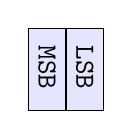
\begin{tikzpicture}[node distance=-\pgflinewidth]                                                                   
\node[short] (u16msb) {\rotatebox{270}{\ttfamily MSB}};
\node[short,right=of u16msb] (u16lsb) {\rotatebox{270}{\ttfamily LSB}};
\end{tikzpicture}                                                                                                            

\subsection{32 bit integral types ({\ttfamily int32\_t}, {\ttfamily uint32\_t})}
\noindent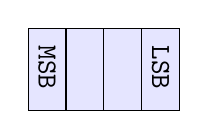
\begin{tikzpicture}[node distance=-\pgflinewidth]                                                                   
\node[short] (u32b1) {\rotatebox{270}{\ttfamily MSB}};
\node[short,right=of u32b1] (u32b2) {};
\node[short,right=of u32b2] (u32b3) {};
\node[short,right=of u32b3] (u32b4) {\rotatebox{270}{\ttfamily LSB}};
\end{tikzpicture}                                                                                                            

\subsection{64 bit integral types ({\ttfamily int64\_t}, {\ttfamily uint64\_t})}
\noindent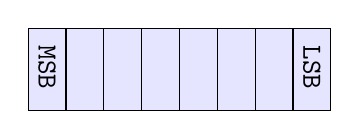
\begin{tikzpicture}[node distance=-\pgflinewidth]                                                                   
\node[short] (u64b1) {\rotatebox{270}{\ttfamily MSB}};
\node[short,right=of u64b1] (u64b2) {};
\node[short,right=of u64b2] (u64b3) {};
\node[short,right=of u64b3] (u64b4) {};
\node[short,right=of u64b4] (u64b5) {};
\node[short,right=of u64b5] (u64b6) {};
\node[short,right=of u64b6] (u64b7) {};
\node[short,right=of u64b7] (u64b8) {\rotatebox{270}{\ttfamily LSB}};
\end{tikzpicture}                                                                                                            

\subsection{\ttfamily float}
\noindent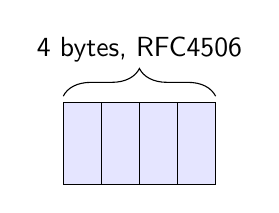
\begin{tikzpicture}[node distance=-\pgflinewidth]                                                                   
\node[short] (u32b1) {};
\node[short,right=of u32b1] (u32b2) {};
\node[short,right=of u32b2] (u32b3) {};
\node[short,right=of u32b3] (u32b4) {};
  \draw[decorate,decoration={brace,raise=2pt,amplitude=1em}] (u32b1.north west) -- node[above=1.1em] {4 bytes, RFC4506} (u32b4.north east);
\end{tikzpicture}                                                                                                            

\subsection{\ttfamily double}
\noindent
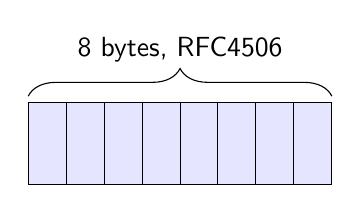
\begin{tikzpicture}[node distance=-\pgflinewidth]
  \node[short] (u64b1) {};
  \node[short,right=of u64b1] (u64b2) {};
  \node[short,right=of u64b2] (u64b3) {};
  \node[short,right=of u64b3] (u64b4) {};
  \node[short,right=of u64b4] (u64b5) {};
  \node[short,right=of u64b5] (u64b6) {};
  \node[short,right=of u64b6] (u64b7) {};
  \node[short,right=of u64b7] (u64b8) {};
  \draw[decorate,decoration={brace,raise=2pt,amplitude=1em}] (u64b1.north west) -- node[above=1.1em] {8 bytes, RFC4506} (u64b8.north east);
\end{tikzpicture}

\subsection{\ttfamily Dwm::SizedLength}
\noindent\begin{tikzpicture}[node distance=-\pgflinewidth]
\node[nineTall,align=center,text centered,,fill=blue!10] (ES) {\Large{\ttfamily ES}};
\node[nineTall,right=of ES] (data1) {\ttfamily data[0]};
\node[dotdot,right=of data1,text width=.6667\textwidth,align=center,text centered] (dots1) {\linebreak \Large{...}};
\node[nineTall,right=of dots1] (data2) {\ttfamily data[size]};
\end{tikzpicture}

\subsubsection{ES (endian, size) byte}

\SizedLengthExample{{},{},{},{},{},{},{},{}}{}{ES byte}

\subsubsection{Examples}
\SizedLengthExample{1,{},{},{},{},0,0,0}{0xAA}{One byte value \texttt{0xAA}, big-endian.}

\SizedLengthExample{0,{},{},{},{},0,0,0}{0xAA}{One byte value \texttt{0xAA}, little-endian.}

\SizedLengthExample{1,{},{},{},{},0,0,1}{0xAA,0xBB}{Two byte value \texttt{0xAABB}, big-endian.}

\SizedLengthExample{0,{},{},{},{},0,0,1}{0xBB,0xAA}{Two byte value \texttt{0xAABB}, little-endian.}

\SizedLengthExample{1,{},{},{},{},0,1,0}{0xAA,0xBB,0xCC}{Three byte value \texttt{0xAABBCC}, big-endian.}

\SizedLengthExample{0,{},{},{},{},0,1,0}{0xCC,0xBB,0xAA}{Three byte value \texttt{0xAABBCC}, little-endian.}

\SizedLengthExample{1,{},{},{},{},0,1,1}{0xAA,0xBB,0xCC,0xDD}{Four byte value \texttt{0xAABBCCDD}, big-endian.}

\SizedLengthExample{0,{},{},{},{},0,1,1}{0xDD,0xCC,0xBB,0xAA}{Four byte value \texttt{0xAABBCCDD}, little-endian.}

\SizedLengthExample{1,{},{},{},{},1,0,0}{0xAA,0xBB,0xCC,0xDD,0xEE}{Five byte value \texttt{0xAABBCCDDEE}, big-endian.}

\SizedLengthExample{0,{},{},{},{},1,0,0}{0xEE,0xDD,0xCC,0xBB,0xAA}{Five byte value \texttt{0xAABBCCDDEE}, big-endian.}

\SizedLengthExample{1,{},{},{},{},1,0,1}{0xAA,0xBB,0xCC,0xDD,0xEE,0xFF}{Six byte value \texttt{0xAABBCCDDEEFF}, big-endian.}

\SizedLengthExample{0,{},{},{},{},1,0,1}{0xFF,0xEE,0xDD,0xCC,0xBB,0xAA}{Six byte value \texttt{0xAABBCCDDEEFF}, little-endian.}

\SizedLengthExample{1,{},{},{},{},1,1,0}{0xAA,0xBB,0xCC,0xDD,0xEE,0xFF,0x99}{Seven byte value \texttt{0xAABBCCDDEEFF99}, big-endian.}

\SizedLengthExample{0,{},{},{},{},1,1,0}{0x99,0xFF,0xEE,0xDD,0xCC,0xBB,0xAA}{Seven byte value \texttt{0xAABBCCDDEEFF99}, little-endian.}

\SizedLengthExample{1,{},{},{},{},1,1,1}{0xAA,0xBB,0xCC,0xDD,0xEE,0xFF,0x99,0x88}{Eight byte value \texttt{0xAABBCCDDEEFF9988}, big-endian.}

\SizedLengthExample{0,{},{},{},{},1,1,1}{0x88,0x99,0xFF,0xEE,0xDD,0xCC,0xBB,0xAA}{Eight byte value \texttt{0xAABBCCDDEEFF9988}, big-endian.}
    
\subsection{\ttfamily std::string}
\LengthEncodedData{uint64\_t}{\texttt{s[0] ... s[length-1]}}{\texttt{std::string} encoding}

\subsection{\ttfamily std::pair<T1,T2>}
\noindent%
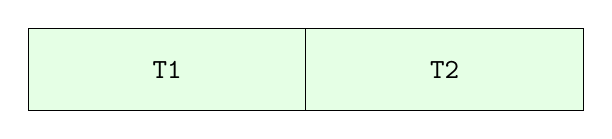
\begin{tikzpicture}[node distance=-\pgflinewidth]
  \node[long] (first) {\linebreak\ttfamily T1};
  \node[long,right=of first] (second) {\linebreak\ttfamily T2};
\end{tikzpicture}

\subsection{\ttfamily std::vector<T>}
\LengthEncodedData{uint64\_t}{\texttt{$T_0$  ...  $T_{length-1}$}}{\texttt{std::vector<T>} encoding}

\subsection{\ttfamily std::deque<T>}
\LengthEncodedData{uint64\_t}{\texttt{$T_0$  ...  $T_{length-1}$}}{\texttt{std::deque<T>} encoding}

\subsection{\ttfamily std::list<T>}
\LengthEncodedData{uint64\_t}{\texttt{$T_0$  ...  $T_{length-1}$}}{\texttt{std::list<T>} encoding}

\subsection{\ttfamily std::map<Key,Value>}
\LengthEncodedData{uint64\_t}{\texttt{std::pair<Key,Value>$_0$  ...  std::pair<Key,Value>$_{length-1}$}}{\texttt{std::map<Key,Value>} encoding}
% \msbencoding{std::pair<Key,Value>}{std::pair<Key,Value>}{entries}

\subsection{\ttfamily std::multimap<Key,Value>}
\msbencoding{std::pair<Key,Value>}{std::pair<Key,Value>}{entries}

\subsection{\ttfamily std::unordered\_map<Key,Value>}
\msbencoding{std::pair<Key,Value>}{std::pair<Key,Value>}{entries}

\subsection{\ttfamily std::unordered\_multimap<Key,Value>}
\msbencoding{std::pair<Key,Value>}{std::pair<Key,Value>}{entries}

\subsection{\ttfamily std::set<T>}
\msbencoding{T}{T}{entries}

\subsection{\ttfamily std::multiset<T>}
\msbencoding{T}{T}{entries}

\subsection{\ttfamily std::unordered\_set<T>}
\msbencoding{T}{T}{entries}

\subsection{\ttfamily std::unordered\_multiset<T>}
\msbencoding{T}{T}{entries}


\end{document}
